\documentclass[10pt,a4paper]{article}
\usepackage[utf8]{inputenc}
\usepackage{amsmath}
\usepackage{amsfonts}
\usepackage{amssymb}
\usepackage{graphicx}
\usepackage[left=2cm,right=2cm,top=2cm,bottom=2cm]{geometry}
\author{Nassime Kabache - Sofiane Atmani - Jean Destribois}
\title{Méthode de Ranking - Compte Rendu}
\date{Mai 2020}

\begin{document}
\maketitle

\section{Introduction}
Le projet effectué dans le cadre du module Méthode de Raking porte sur le calcul du pagerank par la méthode de Gauss Siedel descendant (sujet 5). Le but de ce projet étant de comparer le temps de calcul et le nombre d'itération nécessaire à la convergence entre le calcul du pagerank par la méthode des puissance et le calcul du pagerank par la méthode de Gauss Siedel descendant.


\section{Implémentation}
Le projet contient 4 versions différentes du calcul du pagerank. Voici le détail de ces 4 versions. Pour chacune des 4 versions, un surfeur aléatoire est compris dans le calcul du pagerank et nous arrêtons le calcul lorsque le résultat converge à 0.000001. Nous avons fait le choix d'utiliser le langage C pour programmer ce projet.

\subsection{Version 1}
Cette version est notre version initiale du pagerank. Le stockage de la matrice se fait par ligne. Notre structure de données stock une matrice composée d'un tableau de lignes. Chaque ligne est composé d'un tableau d'éléments. Ces éléments représentent une page web et contiennent le numéro des pages auxquels ils font référence avec leur probabilités.\\
Cette manière de stocker la matrice implique de faire le calcul du pagerank de manière "inverse". En effet, on ne peut pas calculer : 
\[x^{k+1} \lbrack i \rbrack = \sum_{j=1}^{n} x^{k} \lbrack j \rbrack G\lbrack j,i \rbrack\]
car pour un $x \lbrack i \rbrack$ donné, on est pas capable de connaitre les $x \lbrack j \rbrack$ lui faisant référence à moins de parcourir toute la matrice.
On fait donc le calcul de cette manière :
\[x^{k+1} \lbrack G\lbrack i,j \rbrack\ .destination \rbrack = x^{k} \lbrack i \rbrack G\lbrack i,j \rbrack .probabilite\]
\begin{center}
En itérant sur i puis pour chaque i, on itère sur j.
\end{center}

\subsection{Version 2}
Nous avons eu une nouvelle idée pour nous permettre de limiter le coût en mémoire du programme précédent. C'est ce que nous avons implémenté dans cette version. La version 2 fait le calcul du pagerank de la même manière que la version 1. Ce qui diffère est le chargement du fichier dans notre structure de matrice : au lieu de charger toute la matrice, on la charge ligne par ligne pendant le calcul. Cela permet de limiter grandement le coût en mémoire mais ralenti le calcul car pour chaque ligne, on doit faire une lecture de fichier.

\subsection{Version 3}
Nous avons réalisé que la structure de donnée qu'on utilisait pour faire le calcul du pagerank ne pouvait pas fonctionner pour la méthode de Gauss Siedel descendant car à aucun moment dans le calcul d'une itération, on ne peut être certain que $x^{k+1} \lbrack i \rbrack$ a fini d'être calculé. Nous avons donc changé notre structure de données faisant maintenant un stockage en colonne. Ainsi on ne stock plus pour un élément, les éléments auxquels il fait référence mais on stock pour un élément, les éléments qui lui font référence. On calcul donc les $x^{k+1} \lbrack i \rbrack$ de cette manière :
\[x^{k+1} \lbrack i \rbrack = \sum_{j=1}^{n} x^{k} \lbrack j \rbrack G\lbrack j,i \rbrack\]

\subsection{Version 4}
Une fois la version 3 fini, nous nous sommes intéressés au calcul du pagerank par la méthode de Gauss Siedel descendant. C'est ce que nous avons implémenté dans la version 4. On calcul donc les $x^{k+1} \lbrack i \rbrack$ de cette manière :
\[x^{k+1} \lbrack i \rbrack (1 - G \lbrack i, i \rbrack) = \sum_{j=1}^{i-1} x^{k} \lbrack j \rbrack G\lbrack j,i \rbrack + \sum_{j=i+1}^{n} x^{k+1} \lbrack j \rbrack G\lbrack j,i \rbrack\]

\section{Utilisation du programme}
Le projet contient un Makefile permettant d'automatiser la compilation et les différentes exécution du programme. Il contient un fichier README.md dans lequel l'utilisation du programme est détaillé.

\section{Interprétation des résultats}
Tous les résultats que nous mettons ici ont été obtenus sur la même machine. De plus toute la mémoire utilisée pour stocker les matrices a été allouée dynamiquement. Voici les tableaux des résultats :
\\
\\
\begin{center}
Pour une matrice de taille petite (14 éléments non nuls)
\end{center}
\begin{tabular}{| c | c | c | c | c |}
\hline
versions & itérations & temps lecture fichier & temps calcul pagerank & mémoire allouée dynamiquement \\
\hline
1 & 43 & 0.161 ms & 0.154 ms & 656 octets \\
2 & 43 & 0 ms & 0.757 ms & 432 octets\\
3 & 43 & 0.137 ms & 0.471 ms & 624 octets\\
4 & 27 & 0.14 ms & 0.09 ms & 624 octets\\
\hline	
\end{tabular}

\begin{center}
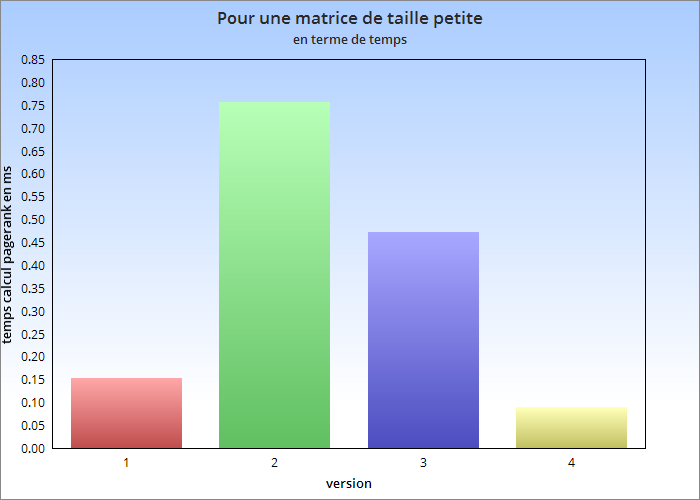
\includegraphics[scale=0.39]{../histogrammes/matrice_petite_temps.png}
\end{center}
\begin{center}
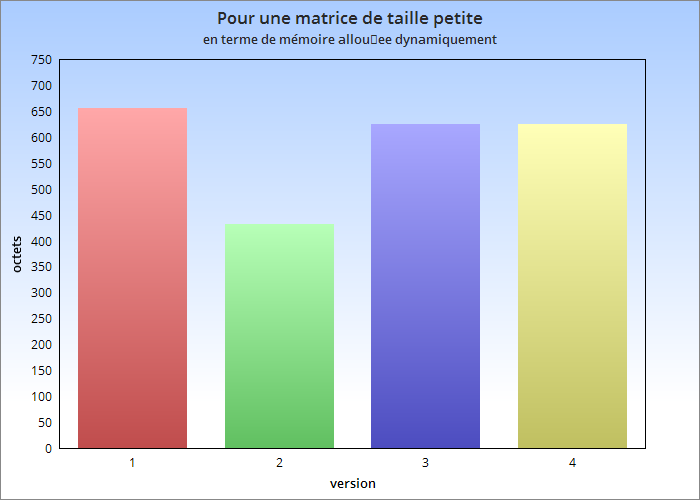
\includegraphics[scale=0.39]{../histogrammes/matrice_petite_memoire.png}
\end{center}

\vspace*{\stretch{1}}
\begin{center}
Pour une matrice de taille moyenne (59995 éléments non nuls)
\end{center}
\begin{tabular}{| c | c | c | c | c |}
\hline
versions & itérations & temps lecture fichier & temps calcul pagerank & mémoire allouée dynamiquement \\
\hline
r1 & 15 & 34.621 ms & 11.241 ms & 1439968 octets \\
2 & 15 & 0 ms & 506.892 ms & 480048 octets\\
3 & 15 & 33.248 ms & 28.571 ms & 1759912 octets\\
4 & 9 & 33.531 ms & 20.494 ms & 1759912 octets\\
\hline	
\end{tabular}

\begin{center}
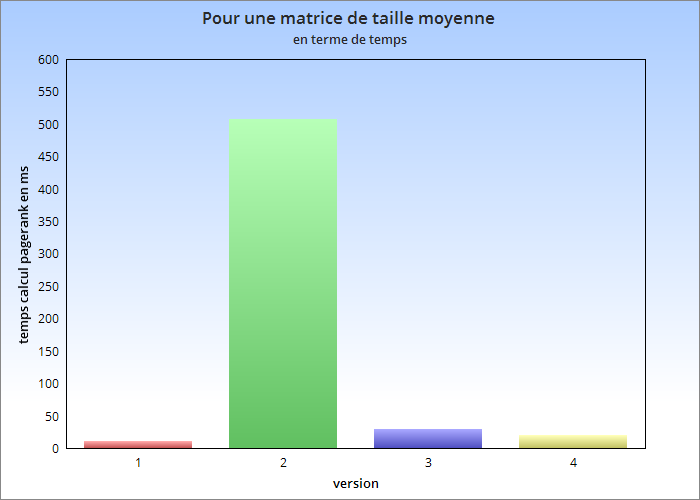
\includegraphics[scale=0.4]{../histogrammes/matrice_moyenne_temps.png}
\end{center}
\begin{center}
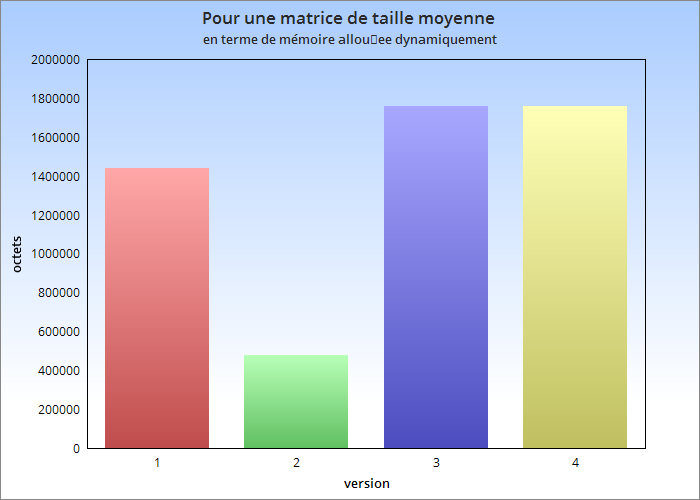
\includegraphics[scale=0.4]{../histogrammes/matrice_moyenne_memoire.png}
\end{center}
\vspace*{\stretch{1}}

\newpage
\begin{center}
Pour une matrice de taille grande (2312497 éléments non nuls)
\end{center}
\begin{tabular}{| c | c | c | c | c |}
\hline
versions & itérations & temps lecture fichier & temps calcul pagerank & mémoire allouée dynamiquement \\
\hline
1 & 65 & 1071.541 ms & 5482.14 ms & 50531296 octets \\
2 & 65 & 0 ms & 63602.972 ms & 13531344 octets\\
3 & 65 & 1354.597 ms & 14068.791 ms & 64520824 octets\\
4 & 35 & 1382.416 ms & 7725.151 ms &  64520824 octets\\
\hline	
\end{tabular}

\begin{center}
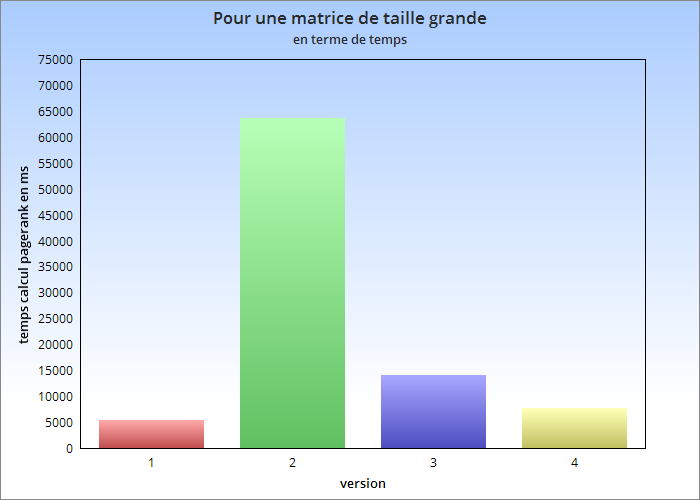
\includegraphics[scale=0.4]{../histogrammes/matrice_grande_temps.png}
\end{center}
\begin{center}
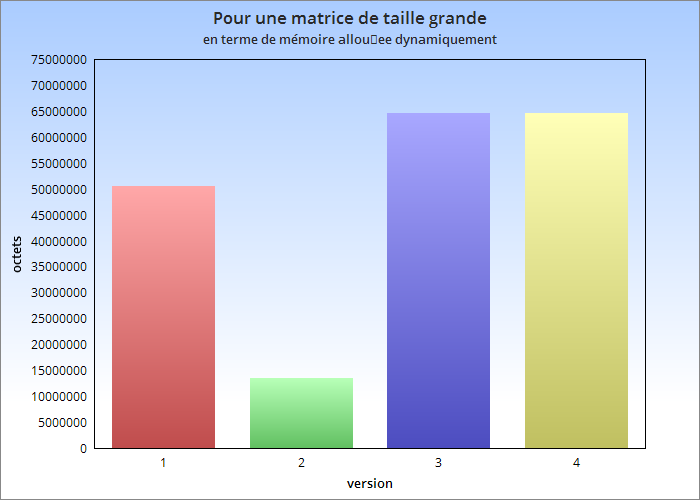
\includegraphics[scale=0.4]{../histogrammes/matrice_grande_memoire.png}
\end{center}

Grâce à ces résultats on voit bien que la version 1, 2 et 3 ont le même nombre d'itérations : ceci est normal car la méthode utilisée est la même. En revanche, pour la version 4, le nombre d'itérations est bien meilleur. On en déduit donc que la méthode de Gauss Siedel descendant améliore (diminue) réellement la quantité de calcul à effectuer pour que la matrice converge. \\
Cependant en ce qui concerne le temps de calcul du pagerank, la version 1 reste la plus rapide. Ceci est probablement dû à une question d'implémentation car la structure de données utilisée est différente. De plus, les nombres correspondants au temps de calcul (et de lecture) ne doivent pas être pris de manière stricte. En effet ces temps peuvent beaucoup varier en fonction de l'occupation de l'ordinateur au moment auquel on exécute le programme. \\
Cependant lorsqu'on observe la version 3 et la version 4 (qui utilisent la même structure de données), on remarque que la version 4 est toujours meilleure en terme de temps de calcul. La méthode de Gauss Siedel descendant améliore donc bien la quantité de calcul et aussi le temps de calcul. \\
On voit également que la version 2 est bien meilleure que toutes les autres en terme de mémoire utilisée. Cependant elle devient très lente  pour une grande matrice dû à la quantité de lecture effectuée ce qui est problématique. \\

\subsection{Conclusion}
La méthode de Gauss Siedel descendant apporte réellement un gain de rapidité et de calcul pour le calcul du pagerank par rapport à la méthode des puissances. Ce projet a été très intéressant pour nous et réellement satisfaisant.


\end{document}